\begin{figure}[H]
    \centering
    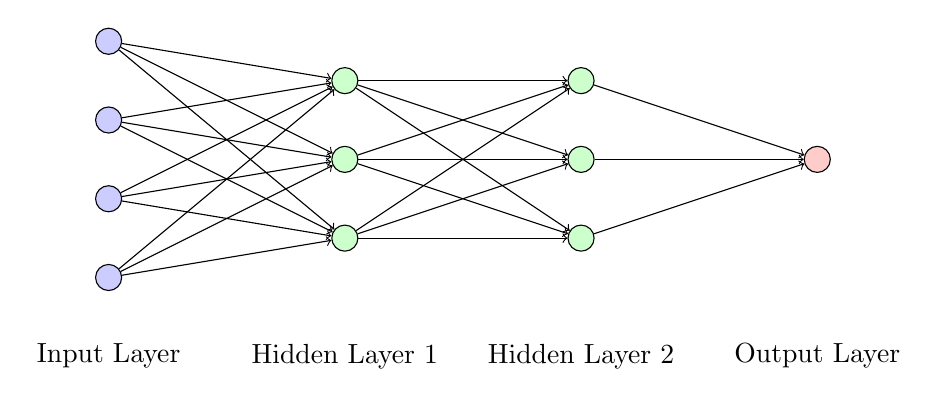
\begin{tikzpicture}
        \node[circle, draw, fill=blue!20] (I1) at (0,3) {};
        \node[circle, draw, fill=blue!20] (I2) at (0,2) {};
        \node[circle, draw, fill=blue!20] (I3) at (0,1) {};
        \node[circle, draw, fill=blue!20] (I4) at (0,0) {};
        \node (I5) at (0,-1) {Input Layer};
        \node[circle, draw, fill=green!20] (H11) at (3,2.5) {};
        \node[circle, draw, fill=green!20] (H12) at (3,1.5) {};
        \node[circle, draw, fill=green!20] (H13) at (3,0.5) {};
        \node (H14) at (3,-1) {Hidden Layer 1};
        \node[circle, draw, fill=green!20] (H21) at (6,2.5) {};
        \node[circle, draw, fill=green!20] (H22) at (6,1.5) {};
        \node[circle, draw, fill=green!20] (H23) at (6,0.5) {};
        \node (H24) at (6,-1) {Hidden Layer 2};
        \node[circle, draw, fill=red!20] (O1) at (9,1.5) {};
        \node (O2) at (9,-1) {Output Layer};
        \foreach \i in {1,2,3,4}
            \foreach \j in {1,2,3}
                \draw[->] (I\i) -- (H1\j);
        \foreach \i in {1,2,3}
            \foreach \j in {1,2,3}
                \draw[->] (H1\i) -- (H2\j);
        \foreach \i in {1,2,3}
            \draw[->] (H2\i) -- (O1);
    \end{tikzpicture}
    \caption{A Deep neural network with two hidden layers.}
    \label{fig:deep-nn}
\end{figure}